\documentclass[tikz]{standalone}
\usepackage{pgfplots}
\pgfplotsset{compat=1.15}
\usepackage{mathrsfs}
\usetikzlibrary{arrows,calc}
\usepackage{tkz-euclide}
\pagestyle{empty}

\definecolor{AngleClr}{rgb}{0,0.39215686274509803,0}
\definecolor{ShapeClr}{rgb}{0.6,0.2,0}

\begin{document}

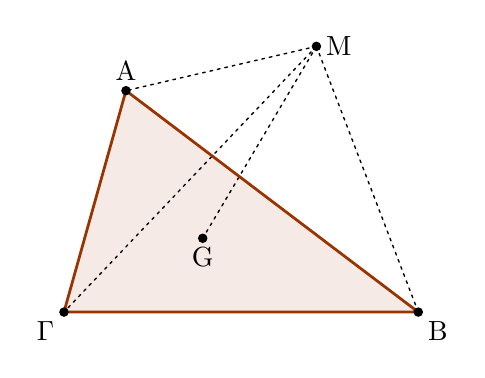
\begin{tikzpicture}[scale=.75]
\tkzSetUpLine[line width=1pt,color=black]
\tkzSetUpPoint[fill=black]

\tkzDefPoints{0/0/A,6/0/B,1.05/3.75/C,4.275/4.5/D}

\tkzDefTriangleCenter[centroid](A,B,C) \tkzGetPoint{G}

\tkzFillPolygon[fill=ShapeClr,fill opacity=0.1,inner sep=1cm](A,B,C)

\tkzDrawSegments[line width=0.5pt,color=black,dashed,dash pattern=on 1pt off 1.75pt](D,A D,B D,C D,G)

\tkzDrawPolygon[color=ShapeClr](A,B,C)
\tkzDrawPoints[size=3](A,B,C,D,G)
\tkzLabelPoint[below left](A){$\rm \Gamma$}
\tkzLabelPoint[below right](B){$\rm B$}
\tkzLabelPoint[above](C){$\rm A$}
\tkzLabelPoint[right](D){$\rm M$}
\tkzLabelPoint[below](G){$\rm G$}

\end{tikzpicture}
\end{document}
